\clearpage
\appendix
\section{Ciclo di Deming (PDCA)}
\label{sec:ciclo_deming}
Ogni processo deve essere organizzato sulla base del Ciclo di Deming, un metodo di gestione iterativo, composto da quattro fasi, utilizzato per il controllo e il miglioramento continuo dei processi e dei prodotti.
Le quattro fasi previste dal ciclo di Deming sono le seguenti:
\begin{itemize}
	\item \textbf{P} - Plan: si stabiliscono gli obiettivi e i processi necessari per fornire i risultati attesi accordati, si assegnano responsabilità, si analizzano cause di criticità e si definiscono azioni di correzione;
	\item \textbf{D} - Do: si attua il piano implementando le attività secondo le linee definite e si raccolgono dati per la creazione di grafici e analisi da destinare alla fase di "Check" e "Act";
	\item \textbf{C} - Check: studio e raccolta dei risultati e dei riscontri. Viene verificato inoltre l'esito delle azioni di miglioramento;
	\item \textbf{A}  - Act: vengono applicate le correzioni necessarie per soddisfare le carenze rilevate e standardizzate le attività.
\end{itemize}
\begin{figure}[h]
	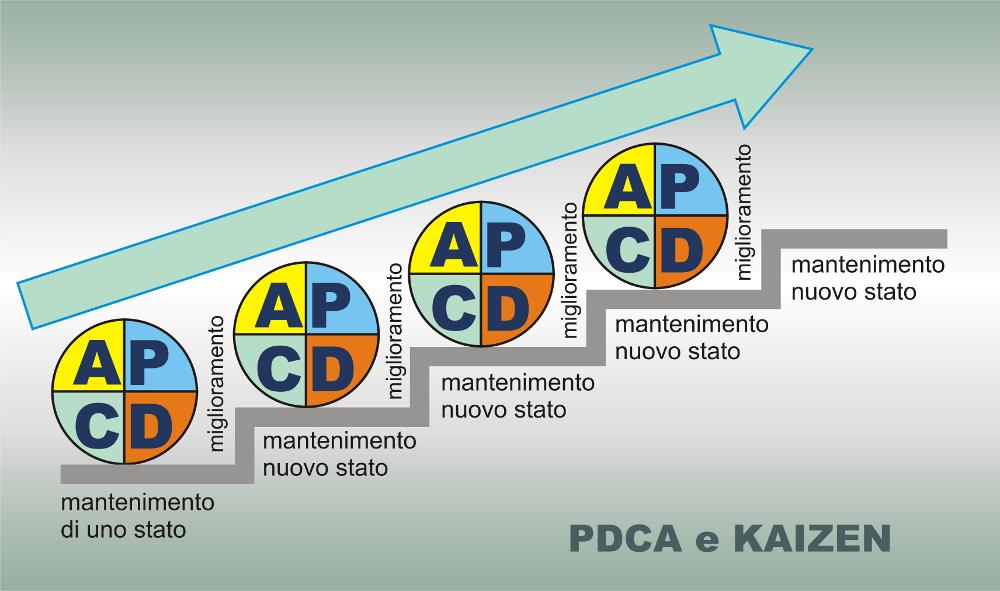
\includegraphics[width=1\textwidth]{../includes/pics/PDCAkaizen.png}
	\caption{Ciclo di Deming PDCA}
\end{figure}
Il metodo PDCA può essere utilizzato inoltre per perseguire il miglioramento continuo, attuando tre cicli evolutivi:
\begin{itemize}
	\item \textbf{Ciclo di mantenimento}: alla base delle fasi di \textit{PLAN} e \textit{DO}, ha la finalità di verificare se quanto pianificato ed attuato continua a dare i risultati attesi. Se il risultato della fase di \textit{CHECK} risulta essere:
	\begin{itemize}
		\item positivo, la fase \textit{ACT} mantiene lo stato attuale;
		\item negativo, allora sarà necessario riattivare il ciclo di azione correttiva.
	\end{itemize}
	\item \textbf{Ciclo di azione correttiva}: qualora l’esito della fase di \textit{CHECK} sia negativo si attua il ciclo di azione correttiva per modificare la situazione del processo. Tale ciclo è caratterizzato da due componenti:
	\begin{itemize}
		\item rimedio, azione immediata finalizzata a correggere;
		\item prevenzione, azione pianificata finalizzata a rimuovere le cause.
	\end{itemize}
	Quando il \textit{CHECK} ritorna ad essere positivo, si attiva nuovamente il ciclo di mantenimento.
	\item \textbf{Ciclo di miglioramento}: tale ciclo presuppone una corretta attuazione dei primi due cicli. Il ciclo di miglioramento viene attuato alla necessità di cambiare, per ottenere risultati ancora migliori,  sul processo attivo. Sarà quindi necessario ripartire dalla fase \textit{PLAN} e continuare con le fasi \textit{DO}, per poi controllare di nuovo con la fase di \textit{CHECK}.
\end{itemize}
\clearpage
\section{ISO/IEC 15504 }
\label{sec:iso}
Nello standard ISO/IEC 15504 specifica come la qualità è strettamente collegata alla maturazione dei processi. Vengono così esposti dei livelli di maturità su cui fare riferimento; il livello più alto corrisponde ad un processo che sarà qualitativamente migliore e maturo.
Lo standard contiene un modello di riferimento che definisce:
\begin{itemize}
	\item Process dimension - dimensione del processo;
	\item Capability dimension - dimensione della capacità.
\end{itemize}
La process dimension comprende i seguenti processi:
\begin{itemize}
	\item Customer/Supplier;
	\item Engineering;
	\item Supporting;
	\item Management;
	\item Organization.
\end{itemize}
La capability dimension definisce una scala di maturità a cinque livelli (più il livello base, detto "livello 0") così definiti:
\begin{itemize}
	\item \textbf{LV 0 - Incomplete process}\\ A questo livello il processo è allo stato iniziale, nelle prime fasi, pertanto non è ancora in grado di svolgere ed adempiere agli obbiettivi per cui è stato creato;
	\item \textbf{LV 1 - Performed process}\\ A questo livello il processo è in grado e ha portato a termine i suoi obbiettivi, ma privo di controllo del lavoro efficace e dettagliato;
	\item \textbf{LV 2 - Managed processs}\\ A questo livello vengono implementate delle prime soluzioni che permettono il controllo del processo, quindi i processi non sono solo funzionanti ma anche monitorati in ogni sua parte;
	\item \textbf{LV 3 - Established process}\\ A questo livello il processo viene definitivamente stabilito;
	\item \textbf{LV 4 - Predictable process}\\ A questo livello il processo viene circoscritto in determinati limiti, in modo tale da essere tenuto ancora più sotto controllo;
	\item \textbf{LV 5 - Optimizing process}\\ A questo livello si è raggiunto uno stato ottimale, il processo viene costantemente tenuto sotto controllo e migliorato per adattarsi alle esigenze del progetto in corso.
\end{itemize}
La capacità (o maturità) dei processi è misurata tramite gli attributi definiti a livello internazionale e che sono:
\begin{itemize}
	\item Livello 1
	\begin{itemize}
		\item \textbf{Process Performance}: capacità di un processo di raggiungere gli obiettivi trasformando input identificabili in output identificabili.
	\end{itemize}
	\item Livello 2
	\begin{itemize}
		\item \textbf{Performance Management}: capacita del processo di elaborare un
		prodotto coerente con gli obiettivi fissati;
		\item \textbf{Work Product Management}: capacità del processo di elaborare un prodotto documentato, controllato e verificato.
	\end{itemize}
	\item Livello 3
	\begin{itemize}
		\item \textbf{Process Definition}: l'esecuzione del processo si basa su standard di
		processo per raggiungere i propri obiettivi;
		\item \textbf{Process Deployment}: capacità del processo di attingere a risorse tecniche e umane appropriate per essere attuato efficacemente.
	\end{itemize}
	\item Livello 4
	\begin{itemize}
		\item \textbf{Process Measurement}: gli obiettivi e le misure di prodotto e di processo vengono usati per garantire il raggiungimento dei traguardi definiti in supporto ai target aziendali;
		\item \textbf{Process Cotrol}: il processo viene controllato tramite misure di prodotto e processo per effettuare correzioni migliorative al processo stesso.
	\end{itemize}
	\item Livello 5
	\begin{itemize}
		\item \textbf{Process Innovation}: i cambiamenti strutturali, di gestione e di esecuzione vengono gestiti in modo controllato per raggiungere i risultati fissati;
		\item \textbf{Process Optimization}: le modifiche al processo sono identificate e implementate per garantire il miglioramento continuo nella realizzazione degli obiettivi di business dell'organizzazione.
	\end{itemize}
\end{itemize}
Ciascuna attributo di processo consiste di una o più pratiche generiche che a loro volta sono elaborate in "Indicatori della pratica" che aiutano nella fase di valutazione delle prestazioni.
Ciascun attributo del processo è valutato secondo una scala a quattro valori (N-P-L-F):
\begin{itemize}
	\item \text{Not achieved (0 - 15\%)};
	\item \text{Partially achieved (>15\% - 50\%)};
	\item \text{Largely achieved (>50\% - 85\%)};
	\item \text{Fully achieved (>85\% - 100\%)}.
\end{itemize}
\begin{figure}[h]
	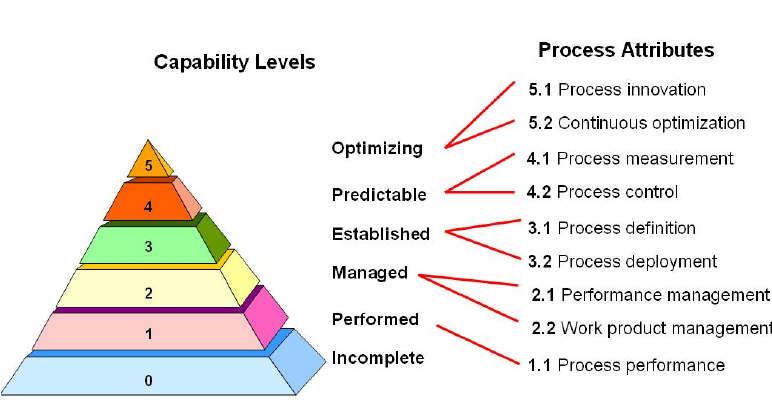
\includegraphics[width=1\textwidth]{../includes/pics/ISO_15504.png}
	\caption{Gerarchia capability dimension ISO 15504}
\end{figure}
